\documentclass{article}
\newcommand{\mc}[1]{\mathcal{#1}}
\usepackage[top=0.8in, bottom=0.8in, left=0.75in, right=0.75in]{geometry}
\usepackage{wrapfig}
\usepackage{subcaption}
\usepackage{graphicx}
\usepackage{amsmath}
\usepackage{amssymb}
\usepackage{caption}

\captionsetup{font=small, width=\linewidth}

\usepackage{titlesec}
\titleformat*{\section}{\large\bfseries}

\usepackage{multicol}

\newlength\tindent
\setlength{\tindent}{\parindent}
\setlength{\parindent}{0pt}
\renewcommand{\indent}{\hspace*{\tindent}}

\begin{document}
\author{Dave Klemish \vspace{-5pt}}
\title{\vspace{-50pt}STA 663 Project: Bayesian Hierarchical Clustering \vspace{-5pt}}

\maketitle

\section{Background}
This project implements the Bayesian agglomerative hierarchical clustering algorithm of Heller and Gharamani \cite{Heller}.  Clustering deals with grouping data such that data in the same group or cluster are more similar (under some criteria).  This problem arises in many diverse fields, including image and document classification, grouping genes into gene families, and partitioning customers into into market segments for advertising purposes.
\\
\\
There are a number of clustering algorithms.  One kind of clustering algorithms are hierarchical clustering algorithms (HCA), which start with a set of unclassified data and then iteratively combines similar data together into clusters.  These algorithms start with each data point as its own separate cluster; then at each iteration the two most "similar" clusters are combined.  The output is a binary tree where each leaf is an individual data point and each node at higher levels in the tree indicate which data points get clustered together based upon their similarity.  
\\
\\
The results of standard HCA procedures depend on the distance metric (a measure of how distance between pairs of data  points) and linkage criteria (a measure of distance between clusters as a function of distances between individual points).  However, there are several distance metrics and linkage criteria that can be chosen, and the final selection between different metrics tends to be made in an ad-hoc manner.  The Bayesian hierarchical clustering (BHC) algorithm addresses this issue by using a probabilistic model of the data, and clustering data together in a probabilistic framework.  The main disadvantage of BHC is its computational requirements compared to distance based clustering methods.

\subsection{Bayesian Hierarchical Clustering}
The main assumption underlying the BHC algorithm is that all data points within a given cluster are generated independently and identically from the same probabilistic model, while data points in different clusters are generated independently from different probabilistic models.  For example, given data $x_i \in \mathcal{R}$, one cluster of data points may all be generated from a Normal(0,1) distribution, while another cluster of data may be generated from a Normal(5,2) distribution.  While these parameters are not actually known, this does not prevent the use of the marginal likelihood of the data from clustering data points together.  By placing a prior on these unknown parameters and then integrating out the parameters, we can obtain the marginal likelihood of the observed data under a given model.  
\\
\\
Let $\mathcal{H}_1^k$ be the model where all data points being considered are generated by the same distribution.  Per equation (1) in Heller, the marginal probability of data $\mathcal{D}_k$ generated from the same distribution is:
\begin{align}
    p(\mathcal{D}_k | \mathcal{H}_1^k) &= \int p(\mathcal{D}_k|\theta)p(\theta|\beta)d\theta \nonumber \\
        &= \int \left[ \prod_{\mathbf{x}^{(i)} \in \mathcal{D}_k} p(\mathbf{x}^{(i)}|\theta)\right] p(\theta|\beta)d\theta
\end{align}
where $p(\theta | \beta)$ is the prior distribution for all parameters of the data generating model, with hyper-parameters $\beta$.  The insight in Heller is that via Bayes' rule, the probability that all data is generated from the same distribution given the data observed is:
\begin{align*}
    p(\mathcal{H}_1^k | \mathcal{D}_k) &= \dfrac{p(\mathcal{D}_k | \mathcal{H}_1^k)p(\mathcal{H}_1^k)}{p(\mathcal{D}_k)}
\end{align*}
Here $p(\mathcal{H}_1^k)$ is the prior probability that all the data comes from the same distribution.  The overall probability of the observed data $p(\mathcal{D}_k)$ is the weighted average of 1) the marginal probability of the data given that all data is from the same model and 2) the marginal probability of the data given that the data comes from two different clusters, weighted on the prior probability $p(\mathcal{H}_1^k)$.  The assumption here is that the alternate model for the data is that it comes from two clusters which are consistent with any merges that have taken place (called tree-consistent partitions in Heller).  Letting $\pi_k = p(\mathcal{H}_1^k)$, which is a function of a hyperparameter $\alpha$, this gives
\begin{align}
       p(\mathcal{H}_1^k | \mathcal{D}_k) &= \dfrac{\pi_k p(\mathcal{D}_k | \pi_k)}{\pi_k p(\mathcal{D}_k | \mathcal{H}_1^k)+(1-\pi_k)p(\mathcal{D}_i | T_i)p(\mathcal{D}_j | T_j)}
\end{align}
This quantity is referred to as $r_k$ in Heller.  The algorithm therefore works as follows:
\begin{enumerate}
\item Initialize each data point as a separate cluster
\item While there is more than one current cluster:
    \begin{enumerate}
    \item For each pair of clusters, calculate $r_k$, the probability these clusters were generated by the same distribution 
    \item Determine which possible combination of clusters has the highest probability $r_k$ of coming from the same distribution
    \item Merge these clusters together
    \end{enumerate}
\item Trim the tree such that only clusters whose probability $r_k$ is greater than some cutoff are kept.
\end{enumerate}

\subsection{Bayesian Hierarchical Clustering for Text Data}
The above discussion is cast in a general framework, where the choice of probabilistic model $p(\mathcal{D}_k|\theta)$ is determined by the problem being considered.  For documents, the standard choice of model is a multinomial model over the entire corpus of words contained in all texts.  Assuming the use of a conjugate Dirichlet prior, the marginal data likelihood in equation (1) reduces to a simple function of sufficient statistics of $\mathcal{D}_k$.  However, Heller does not provide these results, so they are derived as follows:
\\
\\
For multinomial data, the parameter $\theta$ is a $q$-dimensional vector
$\mathbf{p}$ where $k$ is the total number of documents and $q$ is the total number of distinct words in the data.  The
conjugate prior is a Dirichlet distribution with concentration
parameter $\beta$.  Therefore, the pdfs for these distributions are:
\begin{align*}
  p(\mathcal{D}_k | \mathbf{p}) &= \prod_{i=1}^k \left[\dfrac{n_i!}{x_{i1}! \dots x_{iq}!}p_1^{x_{i1}}\dots p_q^{x_{iq}}\right] \\
  p(\mathbf{p} | \beta) &= \frac{1}{B(\beta)}p_1^{\beta_1-1}\dots p_q^{\beta_q-1}
\end{align*}
where $n_i=\sum_j x_{ij}$ is the total word count in document $i$ and $B$ is the multinomial beta function, $B(\beta) =
\dfrac{\prod_{j=1}^q\Gamma(\beta_j)}{\Gamma(\sum_{j=1}^q \beta_j)}$.

It follows that
\begin{align*}
  p(\mathcal{D}_k ,\mathbf{p}|\beta) &= \dfrac{1}{B(\beta)}\left[\prod_{i=1}^k\dfrac{n_i!}{x_{i1}! \dots x_{iq}!}\right]p_1^{(\sum_i x_{i1})+\beta_1-1}\dots p_q^{(\sum_i x_{iq})+\beta_q-1}
\end{align*}
This has the kernel of another Dirichlet distribution, with parameters
$x_1+\beta_1, x_2 + \beta_2, \dots$.  Therefore, we multiply and divide
by the normalizing constant for a Dirichlet distribution with these
parameters.  We can then integrate out the Dirichlet distribution over
$\mathbf{p}$, leaving us with:
\begin{align}
  p(\mathcal{D}_k | \beta) &= \left[\prod_{i=1}^k\dfrac{n_i!}{x_{i1}! \dots x_{iq}!}\right]\dfrac{B(\beta^*)}{B(\beta)} \nonumber \\
    &= \left[\prod_{i=1}^k\dfrac{n_i!}{x_{i1}! \dots x_{iq}!}\right] \dfrac{\prod_{j=1}^q\Gamma(\sum_i x_{ij} +\beta_j)}{\prod_{j=1}^q\Gamma(\beta_j)} \dfrac{\Gamma(\sum_{j=1}^q\beta_j)}{\Gamma(\sum_{j=1}^q \sum_i x_{ij}+\beta_j)} \nonumber \\
    &= \left[\prod_{i=1}^k\dfrac{n_i!}{x_{i1}! \dots x_{iq}!}\right] \dfrac{\prod_{j=1}^q\Gamma(\sum_i x_{ij} +\beta_j)}{\prod_{j=1}^q\Gamma(\beta_j)} \dfrac{\Gamma(\sum_{j=1}^q\beta_j)}{\Gamma(n + \sum_{j=1}^q \beta_j)}
\end{align}
Assuming that $\beta_i$ are constant hyperparameters, their sum can be precomputed to accelerate processing.

\subsection{Programming Implementation of Bayesian Hierarchical Clustering}
The hierarchical structure of the data requires maintaining information about how the tree is built through the iterations of the algorithm.  Therefore, we choose to use a Python class for nodes of the tree, where each node maintains pointers to its child nodes, the number of occurrences of each word in that node, and the probability $r_k$ that the two child nodes are generated from the same probability distribution.  As mentioned above, there is a factor determined by the hyperprior parameters $\beta$ that is needed in the probability calculations at each node; this factor is precalculated and then stored in each node rather than being recalculated during the creation of each node.
\\
\\
Also of note is that equation (3) only works for small problems with limited number of documents and words, since the factorial and gamma functions quickly exceed numeric machine limits as the number of words increases.  Therefore, the Python implementation actually calculates and stores log marginal probabilities.
\\
\\
Our algorithm takes a list of documents encoded as strings, and does some initial text cleansing, including removing punctuation, converting upper case to lower case, and removing common "stop" words that generally impart no meaningful semantic information.  This list of words is copied from the Python Natural Language Toolkit (NLTK) and hard-coded directly into one of our functions; the list was not imported to avoid issues with end-users not having \texttt{nltk.corpus} installed.
\\
\\
All code can be found in https://github.com/dklemish/STA663-Project.

\section{Testing}
In addition to a main function \texttt{BHCmultinomial} that does the actual clustering, there are four additional functions:
\begin{enumerate}
    \item \texttt{clusterNode}: The constructor function for an instance of a clusterNode class.
    \item \texttt{create\_word\_matrix}: Given a corpus of $n$ documents, this function returns a list of all $p$ words contained across all documents as well as a $n \times p$ matrix where entry $i,j$ contains the occurrences of each word $j$ in document $i$.
    \item \texttt{calc\_probability}: Given two clusters of documents, calculate the probability $r_k$ that the documents in each cluster are generated by the same multinomial distribution.
    \item \texttt{merge\_nodes}: Given two clusters, combine the two clusters appropriately into a single new cluster, merging all relevant information.
\end{enumerate}
These five functions are tested using unit tests with \texttt{nosetests}.  A set of three documents is created from a dictionary of three possible words ("cat", "dog", "bird"), plus one additional stopword, where each document contains at most three total words selected from the three possible words.  Based on this data, the correct probabilities and data marginal likelihoods were calculated by hand and compared to the outputs of the functions.  A makefile contained in the \texttt{tests} folder runs all tests.


\section{Application}
This algorithm is applied to a set of 16 documents:
\begin{itemize}
    \item Documents 0-4 are articles about NHL playoff games between the New York Rangers and Pittsburgh Penguins, downloaded from ESPN.com
    \item Document 5 is about the United States Army Rangers
    \item Documents 6 \& 7 are about penguins (the flightless birds found in the Antarctica)
    \item Documents 8-11 are about the Python programming language
    \item Document 12 is about the python species of snakes
    \item Document 13 is about snakes in general
    \item Document 14 is about the Duke Biostatistics department
    \item Documents 15 is the Adventures of Huckleberry Finn by Mark Twain
\end{itemize}
My BHC implementation was run on these documents using hyperparameters of $\beta_j = 1$ for $j=1\dots q$ where the total number of distinct words $q$ is 16,233.  The resulting dendrogram is displayed below in Figure~\ref{fig:BHC}.  Black lines indicate clusters where the probability of clustering nodes together is greater than 0.5, while red lines indicate clusters where the probability of clustering is less than 0.5.  Note that the code to draw the dendrogram is adapted from \cite{Segaran}.
\begin{figure}[h!]
\centering
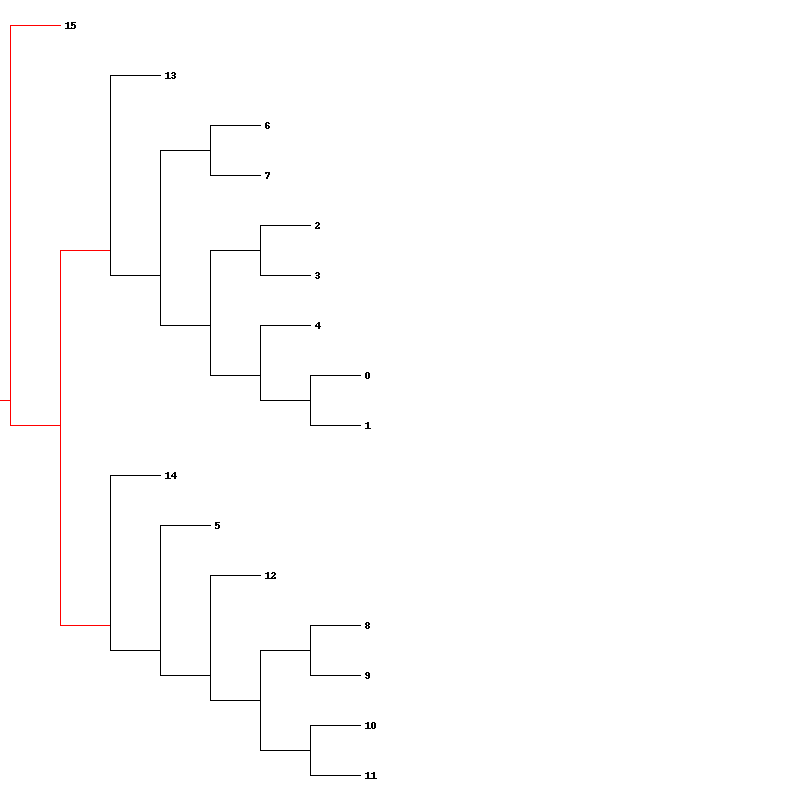
\includegraphics[width=0.75\textwidth]{clusters.png}
\caption{Results of BHC algorithm}
\label{fig:BHC}
\end{figure}
We see that the first groups of documents to get clustered are documents 0-4 on hockey and documents 8-11 on the Python programming language, as these clusters are furthest down in the tree.  After that, the articles on animals (both the general article on snakes and penguins) gets clustered with the hockey articles, presumably based on similarity on the usage of "penguin" and then on other animal related words.  On the other side, the articles on pythons, Army Rangers and the Duke Biostatistics department gets clustered with the Python programming language.  I'm positive there is a joke here somewhere.  
\\
\\
The clustering algorithm rejects the combination of these two clusters as the probability that they are generated from the same multinomial distribution is calculated as being less than 0.5.  Also, Huckleberry Finn is also deemed to be significantly different from the two other clusters.
\\
\\
These results can be sensitive to the choice of hyper-parameter $\beta$ and $\alpha$.  Heller discusses a modification to the BHC algorithm that determines optimal hyperparameters, but I did not implement this modification.
\\
\\
For comparison purposes, Scipy's hierarchical clustering algorithm is run using a Euclidean distance metric and single-linkage clustering (i.e. distance between clusters is the minimum distance of any points between the clusters).  The results are shown below in Figure~\ref{fig:Scipy}.
\begin{figure}[h!]
\centering
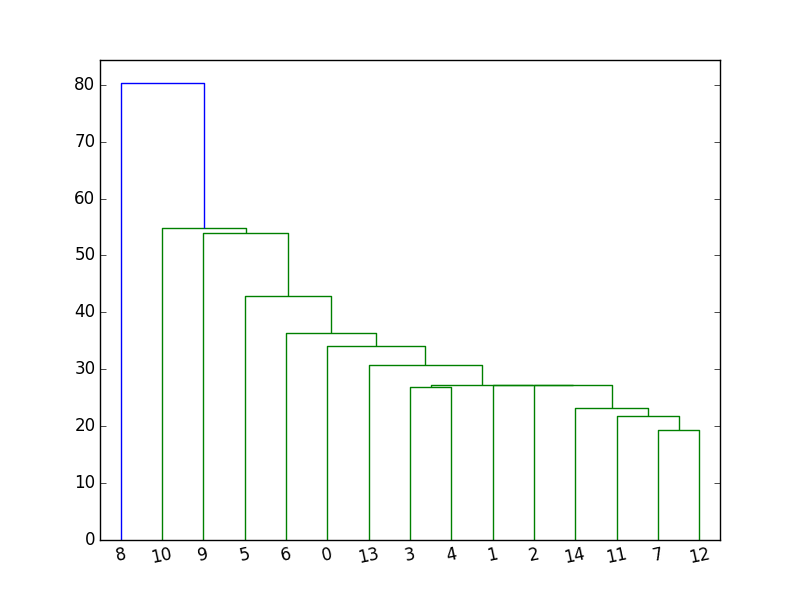
\includegraphics[width=0.75\textwidth]{scipy_cluster.png}
\caption{Results of Scipy's clustering algorithm}
\label{fig:Scipy}
\end{figure}
\\
The results here are not as successful at clustering "similar" (from a human understanding perspective) documents than the BHC algorithm.  The image here is somewhat distorted by the distance between Huckleberry Finn and the other documents, but one of the clusters identified by the algorithm includes the Duke Biostatistics department, an article on penguins, one article on pythons (the snake) and one article on the Python programming language.

\section{Optimization}
The results of running \%prun in an IPython version of this program are displayed below.  The makefile has a line commented out that dumps a full function
profile into a separate \texttt{profile\_results} file, but I wasn't able to either limit the display to only a small number of functions or be in a readable format, so I used \%prun instead.
\begin{verbatim}
    7153303 function calls in 24.991 seconds
        Ordered by: internal time
        List reduced from 36 to 10 due to restriction <10>

        ncalls  tottime  percall  cumtime  percall filename:lineno(function)
        153472   19.703    0.000   19.703    0.000 {method 'count' of 'list' objects}
           711    3.319    0.005    5.093    0.007 bhc.py:9(__init__)
       6984399    0.944    0.000    0.944    0.000 {math.lgamma}
          2167    0.793    0.000    0.793    0.000 {sum}
             1    0.095    0.095   19.847   19.847 bhc.py:77(create_word_matrix)
           862    0.039    0.000    0.039    0.000 {range}
           695    0.027    0.000    4.912    0.007 bhc.py:35(merge_nodes)
            64    0.017    0.000    0.017    0.000 {method 'split' of 'str' objects}
            16    0.016    0.001    0.016    0.001 sets.py:341(_update)
             1    0.012    0.012   24.991   24.991 bhc.py:109(BHCmultinomial)
\end{verbatim}
This program makes a large number of calls to Pythons log gamma function, although each individual call takes almost no time.  The majority of program running time is contained in the count method for list objects.  This is used in my code in the \texttt{create\_words\_matrix} function where the word counts of each document are converted into a list of lists of counts.  This suggests that performance could be improved through use of Cython by eliminating the use of Python lists, but I did not try to implement this as I had enough difficulty getting the algorithm to run in Python.

\begin{thebibliography}{1}

    \bibitem{Heller} Heller, Katherine A and Ghahramani, Zoubin. "Bayesian hierarchical clustering"{\em Proceedings of the 22nd international conference on Machine Learning.} ACM, 2005.
  
    \bibitem{Segaran} Segaran, Toby.  {\em Programming Collective Intelligence: Building Smart Web 2.0 Applications.} O'Reilly Media, 2007.
\end{thebibliography}

\end{document}
